\chapter{System Architecture}
\label{system-architecture}
Well equipped with all the essential theoretical tools that we need, we can move on to implementing them for the game of Abalone. A first logical step would be to look at the existing software landscape to decide if we can utilize existing tools to speed up development.

\section{Software}
\subsection{Machine Learning Library}
Machine learning projects share many components. Most commonly, that is the declaration of the computational graph and the training of the graph. The libraries not only provide those components but also bring significant optimizations and specialized code for hardware acceleration. Therefore, it is imperative to decide on a suitable library to speed up development by several orders of magnitude.

\begin{figure}
    \centering
    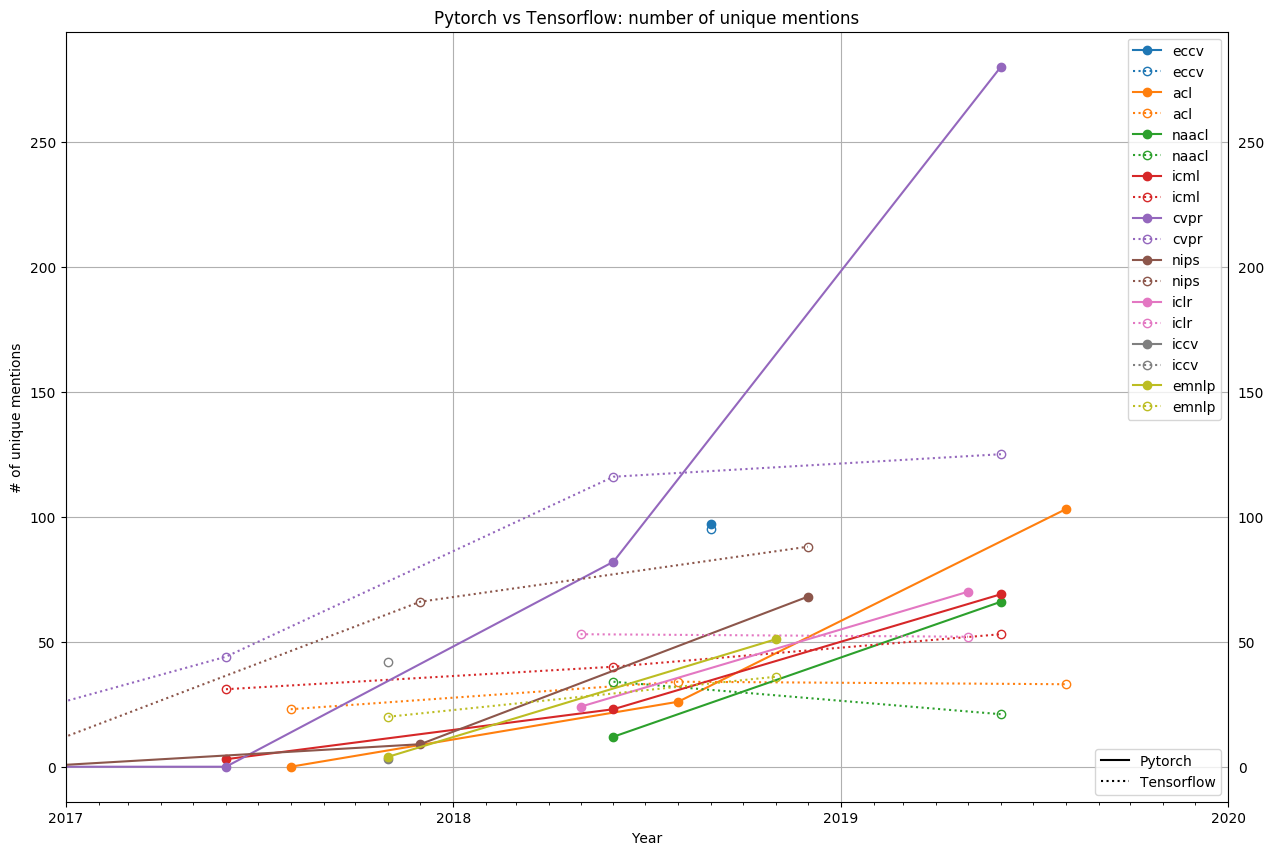
\includegraphics[height=7cm, keepaspectratio]{ml_framework_popularity.png}
    \caption{The mentions of PyTorch and tensorflow in research papers in different publications \cite{noauthor_state_2019}}
    \label{ml_framework_popularity}
\end{figure}

The first indicator to go by is the popularity of the frameworks. The most relevant frameworks are Facebook's PyTorch and Google's TensorFlow. The Keras API has been introduced to TensorFlow, wherefore it is not considered further. In research, PyTorch seems to have quickly taken the dominance as depicted in figure \ref{ml_framework_popularity}. Aside from all differences between both libraries, the choice was guided by two practical reasons. Initially, we selected TensorFlow due to the included support for TPUs as Google granted this project free access to their Research Cloud \cite{noauthor_tpu_nodate}. At a later stage, it became clear that Google was unwilling to increase the CPU quota for the account, limiting the server to 8 cores which posed a significant problem for parallel execution.

In table \ref{PyTorch_vs_tensorflow_performance} there is also a significant performance difference in the inference step of the MCTS. There are two ways in TensorFlow to perform inference, either through the \texttt{predict} function or by calling the \texttt{\_\_call\_\_} method of the $model$ itself. As in the implementation, the inference is not batched but done for individual board states. The usage of the latter option is faster \cite{noauthor_tfkerasmodel_nodate}. Nevertheless, PyTorch is about five times faster. As discussed later, this is the reason to pivot to PyTorch as a framework.

\begin{table*}
    \begin{center}
        \begin{tabular}{ c|c|c|c|c }
            HW  & Framework & Neural net size & $\texttt{predict}(s)$ & $\texttt{\_\_call\_\_}(s)$ \\
            \hline
            \hline
            CPU & tf        & small           & ~0.027s               & ~0.011s                    \\
            GPU & tf        & small           & ~0.024s               & ~0.005s                    \\
            CPU & tf        & large           & ~0.027s               & ~0.015s                    \\
            GPU & tf        & large           & ~0.025s               & ~0.011s                    \\
        \end{tabular}
    \end{center}
    \caption{The average time ($n = 3,000$) taken to perform the feed-forward through the network for state $s$ with either ($\texttt{predict}(s)$) or ($\texttt{\_\_call\_\_}(s)$) in tensorflow}\label{tensorflow_predict_vs_call}
\end{table*}

\begin{table*}
    \begin{center}
        \begin{tabular}{ c|c|c|c|c }
            HW  & Framework & Neural net size & $\texttt{predict}(s)$ & $\texttt{search}(s)$ \\
            \hline
            \hline
            CPU & tf        & small           & ~0.01s                & ~0.016s              \\
            GPU & tf        & small           & ~0.005s               & ~0.011s              \\
            CPU & tf        & large           & ~0.014s               & ~0.02s               \\
            GPU & tf        & large           & ~0.011s               & ~0.017s              \\
            CPU & PyTorch   & small           & ~0.005s               & ~0.011s              \\
            GPU & PyTorch   & small           & ~0.001s               & ~0.007s              \\
            CPU & PyTorch   & large           & ~0.005s               & ~0.011s              \\
            GPU & PyTorch   & large           & ~0.002s               & ~0.008s              \\
        \end{tabular}
    \end{center}
    \caption{The average time ($n = 3,000$) taken to perform the feed-forward through the network for state $s$ ($\texttt{predict}(s)$) and one iteration of MCTS ($\texttt{search}(s)$)}\label{pytorch_vs_tensorflow_performance}
\end{table*}

\subsection{Training Framework}
\label{training_framework}
As there are existing frameworks that have implemented the system described in the AlphaZero paper in a more general and adaptable fashion, it has to be considered building on their foundation:
\begin{itemize}
    \item AlphaZero General is a framework developed as a university project at Stanford originally for the game of Hex and Othello. \cite{thakoor_learning_nodate,thakoor_suragnairalpha-zero-general_nodate}.
    \item Deep MCTS is a framework developed in the context of a Master's thesis \cite{bruasdal_deep_2020,henribru_deep_2021}.
\end{itemize}

We considered a catalog of criteria to compare both options. Parallel training and parallel search measure whether the software implements the parallel training pipeline and MCTS-APV proposed by the AlphaZero paper. Moreover, we checked whether the libraries are agnostic to the game and ML library. Lastly, it is relevant to investigate whether other users could verify the performance.

\begin{table*}
    \begin{center}
        \begin{tabular}{ c|c|c }
            Criterion             & AlphaZero General & Deep MCTS \\
            \hline
            \hline
            Parallel training     & 0                 & 1         \\
            Parallel search       & 0                 & 0         \\
            ML library agnostic   & 1                 & 0         \\
            Game library agnostic & 1                 & 1         \\
            Verified performance  & 1                 & 0         \\
            Simplicity            & 1                 & 0         \\
            \hline
            \hline
            Sum                   & 4                 & 2         \\
        \end{tabular}
    \end{center}
    \caption{A comparison of existing AlphaZero frameworks}\label{training_framework_comparison}
\end{table*}

As shown by table \ref{training_framework_comparison}, the winner by those criteria is AlphaZero General. The core advantages of the library are its simplicity and popularity. Deep MCTS makes use of a lot of abstractions and generics, which makes the code more professional and reusable. Nevertheless, this also poses significant difficulties in understanding. The application of AlphaZero General to multiple other games like Gobang, Santorini, Connect4, and more has shown its performance. The major drawback is the lack of a parallelized training pipeline.

\subsection{Game Engine}
There are multiple relevant implementations of game engines for Abalone. As the interfacing language for PyTorch is Python, it makes sense to restrict the engines to Python:

\begin{itemize}
    \item Abalone-BoAI is a game engine specifically designed for interfacing with computational agents. It is straightforward and has been used for the precursor project of this thesis \cite{scriptim_scriptimabalone-boai_2021}.
    \item Gym-abalone is tightly integrated with OpenAI's gym, potentially allowing agents to play other games as well. The API is suited for the reinforcement learning setting \cite{towzeur_towzeurgym-abalone_2021}.
\end{itemize}

Two arguments lead to the decision of choosing Abalone-BOAI:
\begin{enumerate}
    \item We already optimized it in the previous project, like the generation of legal moves.
    \item The API of the engine needs to be adapted to fit the interface of the training framework. Both engines are stateful, meaning that they rely on the class instance context to perform moves, check for legal moves, and other operations. AlphaZero General expects the game engine to be designed in a functional way. For instance, the operations are supposed to be applied to the input matrix, and the modified matrix is then returned. Therefore, intricate knowledge of the engine is of advantage.
\end{enumerate}

Due to those necessary modifications, the original game engine was forked to allow for more accessible packaging \cite{campfireman_campfiremanabalone-boai_2021}.

\begin{figure}
    \centering
    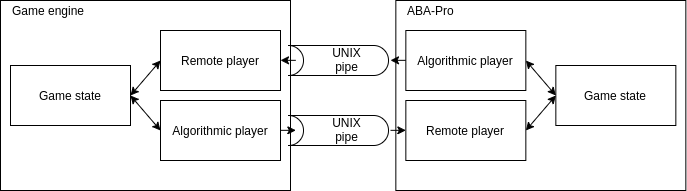
\includegraphics[height=4cm, keepaspectratio]{game_engine_communication.png}
    \caption{The inter process communication between the python game engine and the Java implementation of ABA-PRO}
    \label{python_java_ipc}
\end{figure}

As mentioned in the section \ref{existing_game_playing_agents}, Verloop's reimplementation \cite{verloop_abaloneai_nodate} offers the simplest solution for interfacing with (one of) the strongest Abalone algorithms. In a small tournament, personal implementations of minimax in Python \cite{claussen_abalone_2021} were inferior. As the Java implementation is tightly coupled with the internal game engine, we decided to implement a proxy player for each game engine. Each engine is a separate process, and the proxy players relay the moves between the engines. The proxy players communicate through a named pipe as depicted in figure \ref{python_java_ipc}. The downside of this solution is the need to synchronize two separate game states and translate between the different move notations. We used the notation introduced in section \ref{abalone_move_notation} to serialize the moves.


\section{Neural Network}
\subsection{Dimensions}
In order to apply the neural network architecture proposed by AlphaZero (cf. figure \ref{alpha_zero_neural_network}) two dimensions need to be changed:
\begin{enumerate}
    \item The input matrix of size $19 \cdot 19 \cdot 17$ needs to be adjusted to fit the dimensions of the hexagonal board. The hexagonal board is transformed into an orthogonal base as shown in \ref{abalone_matrix_representation} such that it can be represented as a $9 \cdot 9$ matrix.
          The third dimension of size $17$ can be reduced to 1 by removing the move history and only passing the current state. By representing the state as proposed in \ref{board_representations}, there are no separate planes necessary. Additionally, the board is always passed in its canonical form to the network. The board states are always seen from black's perspective in the canonical form. If it is the black player's turn, the board remains unchanged. If it is white's turn, the board's colors are switched. From the perspective of the neural network, white ($-1$) is always the opponent. The in-turn player is represented as $1$ and $-1$ for black and white. The matrix values can be multiplied with the in-turn player value to create the canonical form.
    \item AlphaZero's output vector $\pi$ of size 381 represents all possible positions a piece can be placed on the board. As Abalone has a much more complex move system, the size of this vector needs to match the number of all possible moves. We found the number of all possible moves by generating all moves programmatically. The generated moves were stored in a bijective map. Each move is assigned an index in $\pi$ and represented as a string in the proposed notation above. Therefore, using the bijective map, a move's index can be found by its string representation and vice versa.

          As depicted in figure \ref{possible_move_generation_inline}, the inline moves are generated by iterating over all fields of the board. For each field, all directions are tested for being a valid move. If that is the case, the move is added to the bijective map. In case the move is already in the map, the move is skipped.

          \begin{figure}
              \centering
              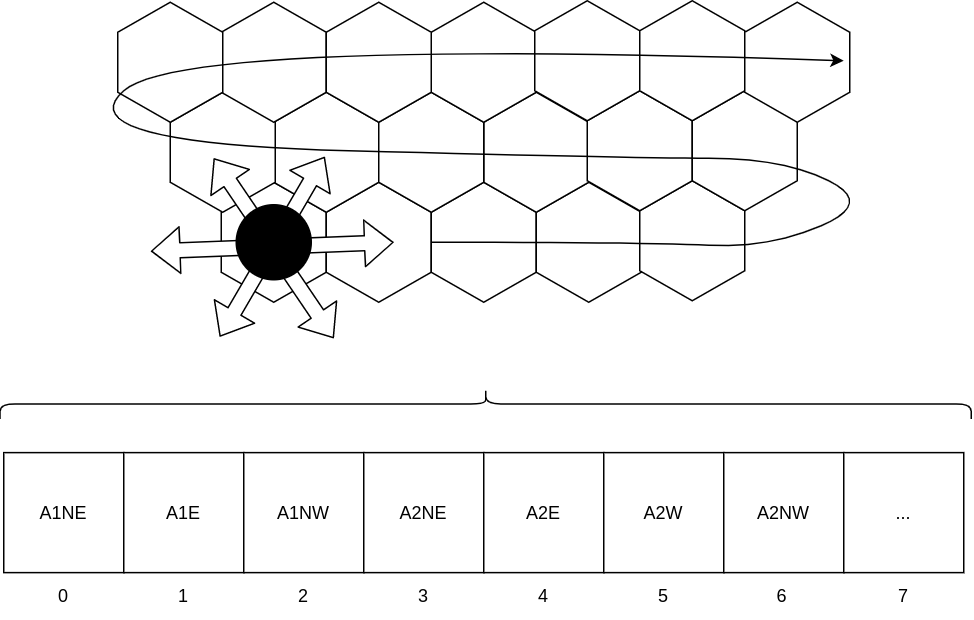
\includegraphics[width=12cm, keepaspectratio]{possible_move_generation_inline.png}
              \caption{Generation of inline moves, starting at position A1 and direction NE}
              \label{possible_move_generation_inline}
          \end{figure}

          Figure \ref{possible_move_generation_broadside} shows the generation of the broadside moves. The algorithm iterates each field. For each field, marble lines of length two and three are generated in all (possible) directions. For each line broadside in all directions, moves are checked for validity. The move direction of the marble line direction is ignored.

          \begin{figure}
              \centering
              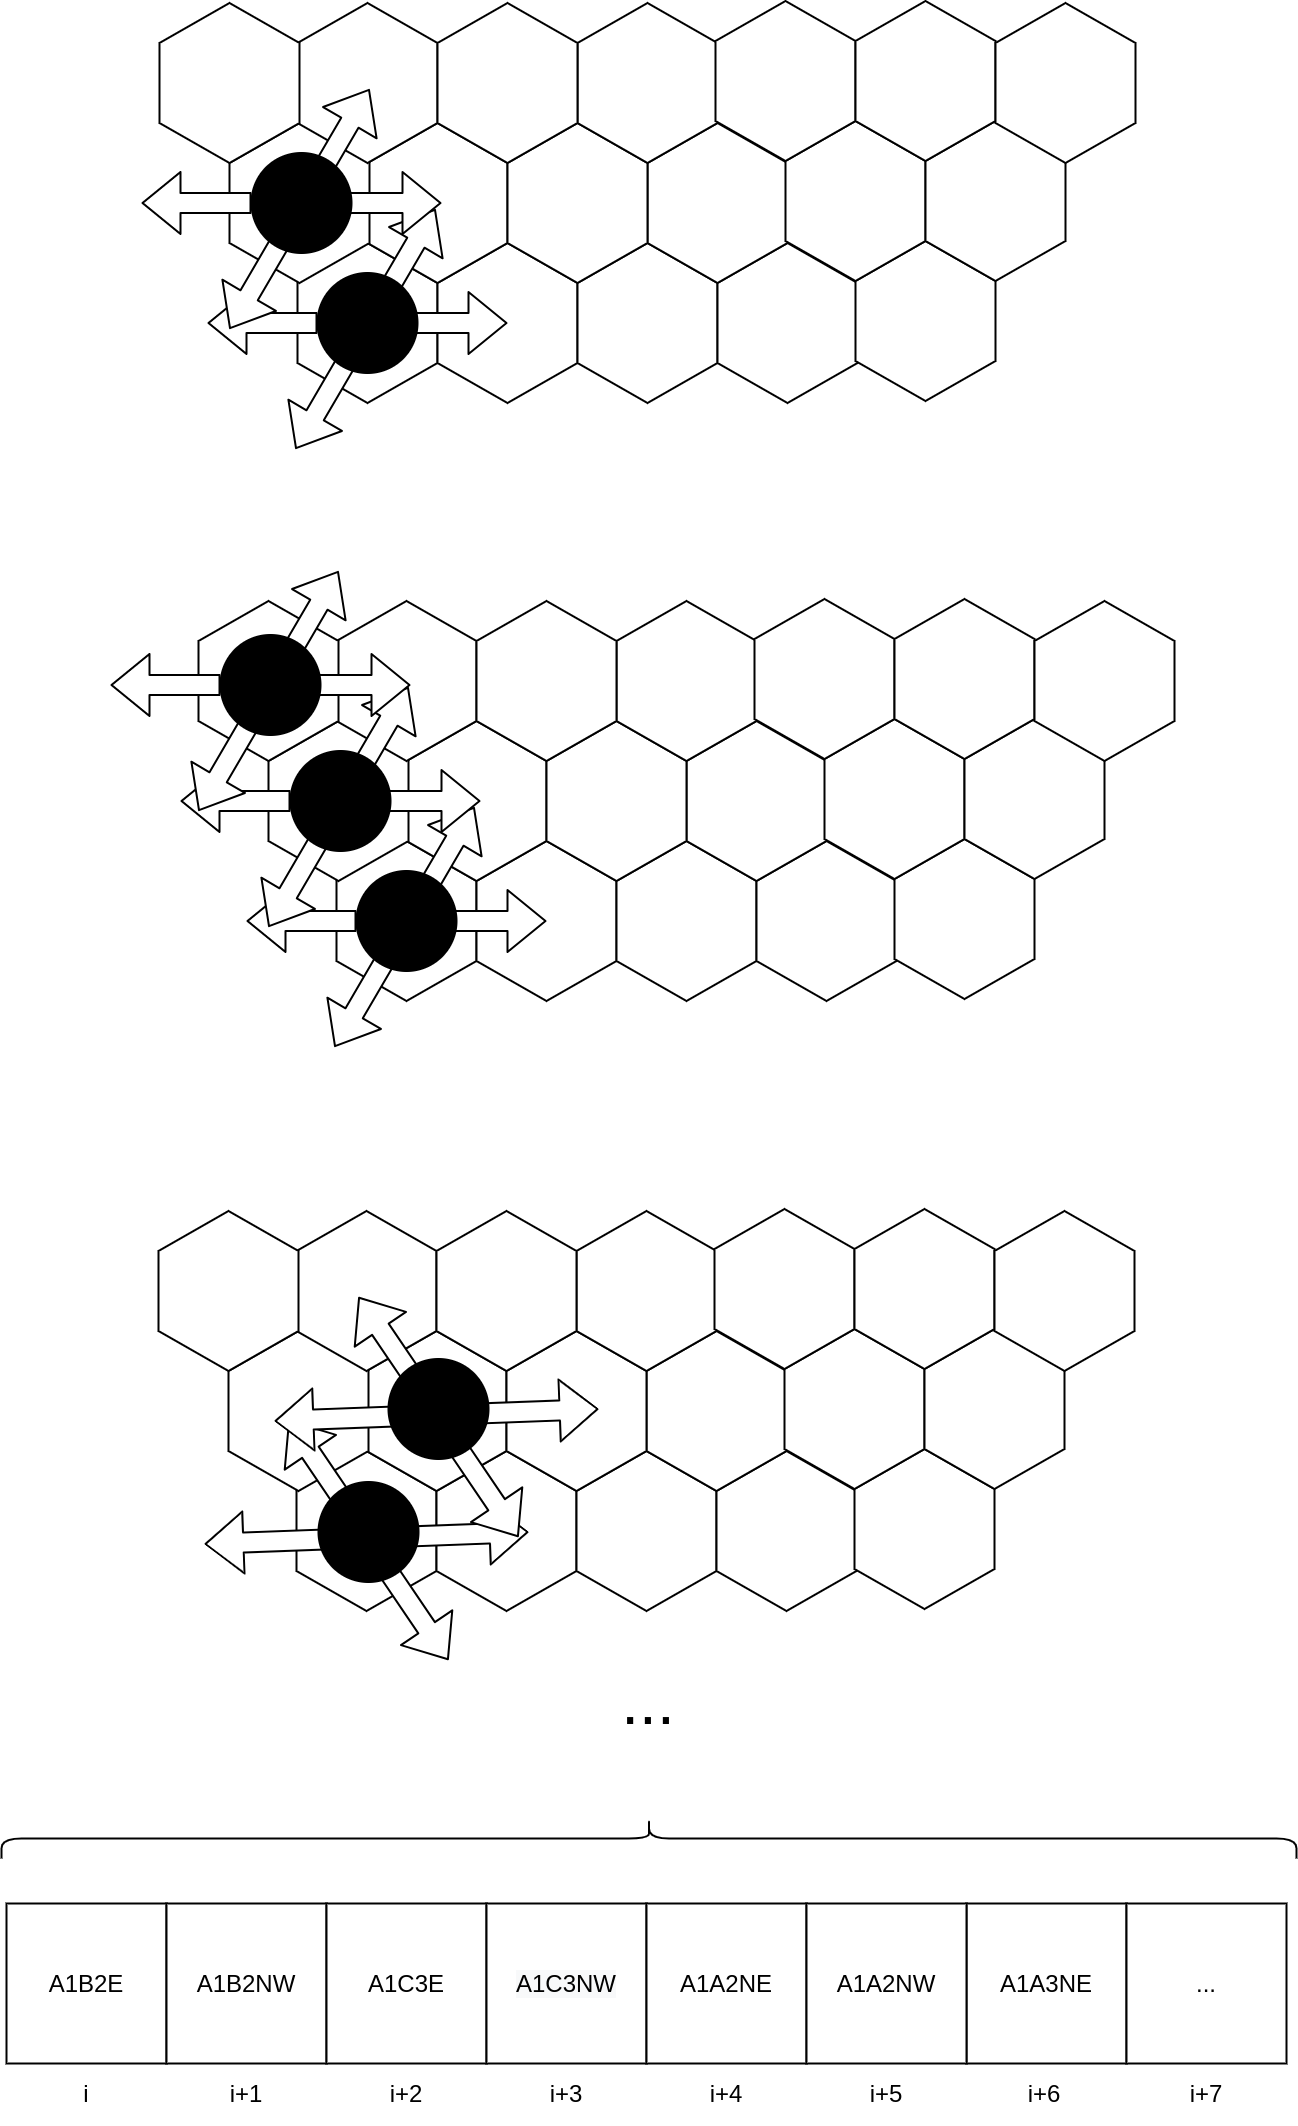
\includegraphics[width=12cm, keepaspectratio]{possible_move_generation_broadside.png}
              \caption{Generation of broadside moves starting at position A1, line direction NE, line length of two and at move direction NE}
              \label{possible_move_generation_broadside}
          \end{figure}

          The resulting vector $\pi$ has a length of $1452$.
\end{enumerate}

\subsection{Architecture}
% explain pi and v
\section{Training Pipeline}
\subsection{Components}
\label{components}

The training pipeline of AlphaZero General has five main components:
\begin{enumerate}
    \item \textbf{Coach}: The main module that orchestrates the training process.
    \item \textbf{game}: Provides an abstract interface that generalizes to many types of board games. Functions like the generation of legal moves, creating a unique string representation of the board, and other functions need to be implemented.
    \item \textbf{Neural Net}: Is a wrapper for any neural network. It needs to be implemented for the specific framework used.
    \item \textbf{MCTS}: Encapsulates the logic to perform Monte Carlo Tree Search on the game tree with the help of the neural network and the Game module.
    \item \textbf{Arena}: Has the task to perform the face-off between different agents.
\end{enumerate}

Aside from the modifications made to parallelize the framework in section \ref{parallelization}, we made multiple modifications.
\begin{itemize}
    \item The Arena was modified to use the Abalone engine \cite{claussen_abalone_2021} and game-playing agents implemented for that engine. This way, the neural nets can be faced off against other algorithms like Verloop's minimax.
    \item Moreover, the MCTS implementation could not deal with games with board states appearing multiple times in the search tree. The implementation uses hash maps to retrieve the action-values and counts for a board state. If the board state exists multiple times in the search tree, the values are skewed. We extended the hash of a state by a hash of the parent node's hash and the current depth of the node to solve the problem.
    \item Lastly, the Arena was parallelized because the face-off with a random agent or a previous version requires a more significant number of games to get a statistically relevant result. As discussed in section \ref{parallelization}, the significant length of a game would slow down the training process too much.
\end{itemize}

Additionally, we added a CLI entry point to pass arguments to the training process. All relevant hyperparameters of a training run are persisted in a JSON file. Performance data, such as time per iteration, and the Arena results are logged as CSV tables.

\subsection{Algorithm}
Even though we alter the main training routine later to be executed in parallel, the logic remains quite similar to the original algorithm devised in AlphaZero General. Therefore, it makes sense to describe the coarse structure that is also outlined in figure \ref{training_algorithm}.

The outer loop defines how many iterations of self-play and subsequent neural network training should be performed. At the beginning of each iteration, a predefined number of episodes is supposed to be played.

In each episode, an MCTS is performed with the defined number of simulations. The temperature parameter $\tau$ determines the exploration: Either a move is selected with a probability proportional to the number of visits, or the move with the highest count is selected. The move is applied to the board state. After switching the sides, it is checked whether a terminal state was reached. If not, the game is continued. Otherwise, the reward $r$ is calculated. With $r$, the list of experiences $(s, \pi, z)$ is generated, with $z$ being the reward $r$ from the perspective of the player in turn.

After the desired number of games has been played, the new experience is appended to the experience buffer. Moreover, the buffer is stored as a checkpoint. If the buffer exceeds a defined length, the oldest experience is removed. Then a new version of the network $f_{\theta}$ is trained and played against the previous version in the Arena. If the new network performs better than the previous version, it is stored on disk for checkpointing. Otherwise, the network is discarded. The training is then continued until the desired number of iterations is reached, or the training is aborted.

\begin{figure}[H]
    \centering
    \subfloat[The main loop of the training algorithm]{
        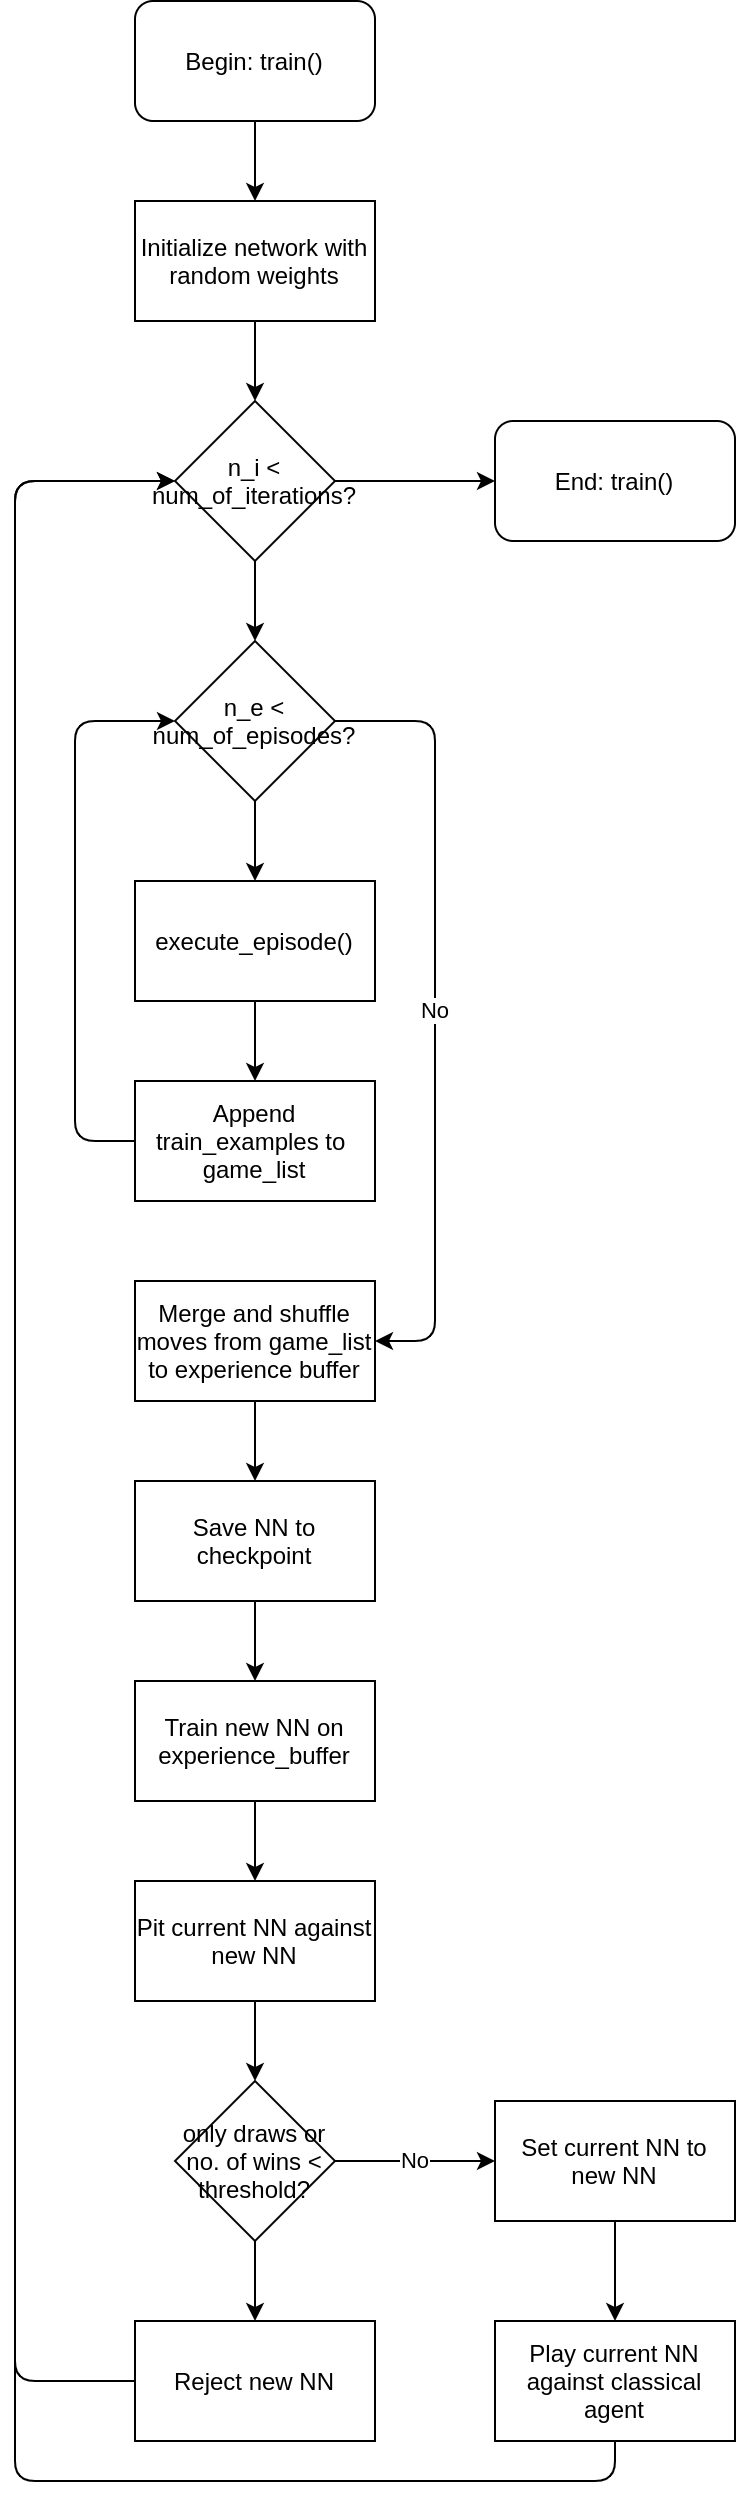
\includegraphics[height=19cm, keepaspectratio]{training_main_loop.png}
    }
    % \hfill
    \subfloat[The episode loop]{
        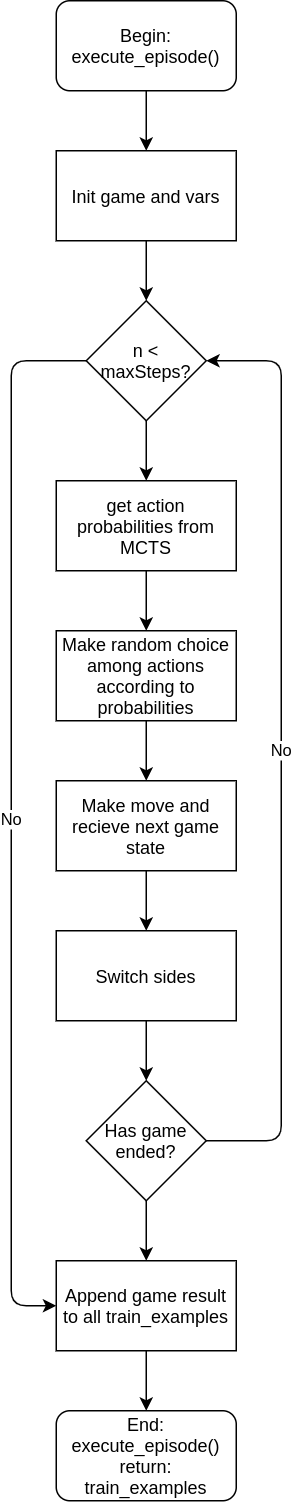
\includegraphics[height=19cm, keepaspectratio]{training_episode.png}
    }
    \caption{The self-play training pipeline}
    \label{training_algorithm}
\end{figure}

\subsection{Parallelization}
\label{parallelization}
AlphaZero General's training pipeline does not offer parallel training. By comparing the time taken to execute one episode for the game of Othello and Abalone, it showed that a game of Abalone takes on average $40$ times (n=100) longer to finish: 1s for Othello and 40s for Abalone. Investigating potential improvements, it became clear that there are two major factors that determine the runtime of an episode:

1. Length of the game. A game of Abalone takes significantly more turns, caused by rules not forbidding loops such that games can be infinite. Moreover, defensive play styles can draw out games significantly. By limiting number of turns $m$ per game and evaluating the state of the game at that step, the issue can be alleviated. In this case, the length was limited to $m=200$.

2. The MCTS being computationally expensive: A closer inspection of the execution time, holding all variables constant, demonstrates the culprit. The simulation step of MCTS uses the neural network. The time taken by this function is one order of magnitude larger than the second most expensive operation, which is the generation of legal moves. For example, when running 15 MCTS iterations with the original TensorFlow implementation, one turn takes

\begin{itemize}
    \item Total time: 0.44s
    \item One MCTS iteration: 0.03s
    \item Neural network : 0.025s
    \item Valid move generation: 0.05s
\end{itemize}

Looking at the main variables that control the length of the nested loops, it becomes clear that reducing the time an MCTS iteration takes is essential. Assuming function $f$ is the operation to perform one Monte Carlo simulation:

$$
    k := \text{number of games}
$$
$$
    m := \text{number of turns per game}
$$
$$
    n := \text{number of MCTS simulations}
$$
$$
    f \in O(kmn)
$$

Abalone requires a larger number of MCTS simulations. The other projects \cite{bruasdal_deep_2020,thakoor_learning_nodate} used only 30 iterations for Othello and Hex, but Abalone has a much more complex game tree. AlphaZero performs $1,600$ iterations \cite[p. 11]{silver_mastering_2017} for each move. For the network to improve, the MCTS needs to recommend a better move than the pure network. It is the policy improvement operator. Those propties were the reason to decide to use PyTorch. The library brings a $5$-times improvement for that step as shown in \ref{pytorch_vs_tensorflow_performance}. Nevertheless, this only brings down execution time for one episode by a factor of $5$, still being $8$-times slower than the reference implementation for Othello. AlphaZero uses two ways to alleviate this problem:

\begin{itemize}
    \item Parallelization of the self-play training
    \item Parallelization of the MCTS (APV-MCTS)
\end{itemize}

As Python's global interpreter lock \cite{noauthor_globalinterpreterlock_nodate} doesn't allow for true multithreading, parallelizing the MCTS poses significant complexity and difficulty. However, allowing for simultaneous self-play and training of the neural network is feasible. As already mentioned in section \ref{training_framework}, the implementation by Bruåsdal \cite{bruasdal_deep_2020} provides this feature. For that reason its architecture is used as a blueprint for migrating AlphaZero General into a parallel architecture. The figure \ref{parallel_training_pipeline} depicts how the components mentioned interact in a parallel fashion.

\begin{figure}[H]
    \centering
    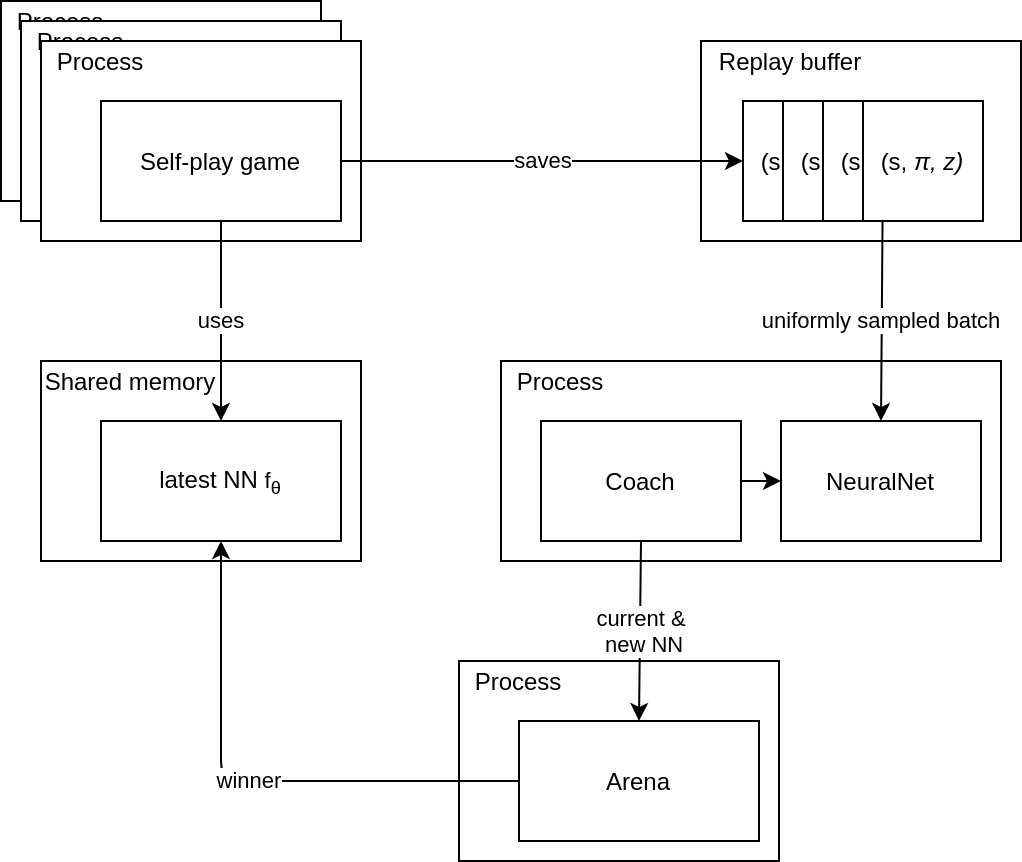
\includegraphics[height=10cm, keepaspectratio]{parallel-training.png}
    \caption{The different processes during the parallel training \cite[cf. p. 45]{bruasdal_deep_2020}}
    \label{parallel_training_pipeline}
\end{figure}

There are multiple self-play workers that use the current best neural network $f_{\theta}$ to generate experience. The experience is put into a queue to allow for asynchronous communication between the worker processes and the Coach. For each training iteration of the neural network, the queue is emptied and loaded into the replay buffer. If the experience buffer exceeds the maximum size, the oldest experience is dropped. The number of training batches is defined by the batch size and buffer size (buffer size divided by batch size). The training batches are created by randomly sampling tuples ($s, \pi, z$) from the buffer. No tuple is used twice, so that the entire buffer is utilized.

After training the neural network with the batches, the newly created network is pitted against the old version in the Arena. As both variants are pitted against each other multiple times, the Arena is parallelized as well. If the new network is stronger, it is saved on disk and a version counter is incremented. The version counter is a shared variable between the workers and the Coach. After each completed self-play game the worker checks if the version counter is larger than its stored version. If that is the case, the new network is loaded from disk.

An important factor is to balance the amount of workers against the time it takes to train the neural network. If the buffer grows large, training takes a long time. In the meantime a lot of new experience is potentially generated. This then overrides all previous experience, such that all experience is only generated from one network. This might make the training process less robust.

\subsection{Symmetrical Board Generation}
Abalone's board has six rotational symmetries and six mirror axes, as mentioned in \ref{state_space_complexity}. That means $\pi$ and $v$ are equivalent for up to 12 symmetrical board states. By generating the symmetrical board states for each tuple ($s, \pi, z)$, the data can be augmented by a factor of twelve. There are some board configurations in which there are less symmetrical boards as some are identical. For example, rotating the default starting position by 120° produces the same board as mirroring it by the $s$ axis. In general, the factor of 12 does hold for almost all board states.

To create the additional experience the positions of the marbles are turned into cube coordinates. For cube coordinates there is a simple way to mirror coordinates and also to rotate coordinates. A mapping function transforms marble coordinates from their matrix coordinates of the form $(x, y)$ to the form of $(q, r, s)$. The origin of the cube coordinate system is laid into the center of the Abalone board, such that e.g. $E5 = (0, 0, 0)$ or $A1 = (-4, 4, 0)$.

The transformed coordinates can be rotated around the origin by 60° clockwise by shifting the values to the right and negating the values:

\begin{BVerbatim}
    [ q,  r,  s ]
    to  [-r, -s, -q ]
    to     [  s,  q,  r ]
\end{BVerbatim}

To mirror a cube coordinate along one of the three main coordinate axes $q, r$ or $s$ the two coordinates that don't belong to the axis are swapped:

\begin{BVerbatim}
    function reflect_q(h) { return Cube(h.q, h.s, h.r); }
    function reflect_r(h) { return Cube(h.s, h.r, h.q); }
    function reflect_s(h) { return Cube(h.r, h.q, h.s); }
\end{BVerbatim}

For mirroring along the axis that is orthogonal to the main axis, the coordinates need to be negated first. Besides all marbles, all moves in $\pi$, whose probability is not $0$, have to be transformed as well. First, the move corresponding to the index in $\pi$ is looked up. As a move consists of one or two marble coordinates, those are transformed by the same scheme. The directions can be transformed into cube coordinates as well:

\begin{BVerbatim}
    (+1, -1, 0): NORTH_EAST
    (+1, 0, -1): EAST
    (0, +1, -1): SOUTH_EAST
    (-1, +1, 0): SOUTH_WEST
    (-1, 0, +1): WEST
    (0, -1, +1): NORTH_WEST
\end{BVerbatim}

This way the same functions can be applied to the directions. After all operations are applied the cube coordinates are converted back to marble coordinates and moves. In case of the moves, the probabilities from the original $\pi$ are written to the new index position.

\subsection{Warm-Up}
AlphaZero starts learning from scratch, there is no information about what constitutes a good move or strategy. This creates a cold-start problem, the self-play learning might not improve performance or even harm performance for an extended period of time. Equipped with ample computational resources like DeepMind, this poses no problem and is even desirable: The network is not nudged into a specific direction and can produce more novel insights.

Investigations into the application of AlphaZero's training principle showed possible ways to warm-start the training of the network \cite{wang_adaptive_2021}. Wang proposes an adaptive rollout based warm-start. This reintroduces rollouts into the MCTS that are performed at the beginning of the training process and are slowly phased out over the course of training.

Another possibility would be to essentially reintroduce components of AlphaGo. Either by using a database of moves or alternatively by letting the agent train against a heuristic agent. For Abalone we propose a similar method. By letting a heuristic agent play against a random agent, an initial experience buffer is created. Thus, the first iteration of the training of $f_{\theta}$ produces a function that approximates the heuristic player. It is hypothesized that the self-play then further improves this warmed up agent. This is akin to the RL step in AlphaGo.
